\subsection*{Problema 39}

\textbf{Enunciado:}
Calcular la integral indefinida:
\begin{align*}
\int \dfrac{x^2 \, dx}{(3 + x)^{-5/3}}
\end{align*}

\textbf{Solución:}
Siguiendo las indicaciones, reescribimos el denominador negativo como un exponente positivo en el numerador:
\begin{align*}
I = \int x^2 (3 + x)^{5/3} \, dx
\end{align*}

Aplicamos el cambio de variable sugerido:
\begin{align*}
u &= 3 + x \implies x = u - 3 \\
du &= dx
\end{align*}

Sustituimos estas expresiones en la integral:
\begin{align*}
I &= \int (u - 3)^2 u^{5/3} \, du \\
I &= \int (u^2 - 6u + 9) u^{5/3} \, du
\end{align*}

Multiplicamos aplicando las leyes de los exponentes ($u^2 u^{5/3} = u^{11/3}$, etc.):
\begin{align*}
I = \int \left( u^{11/3} - 6u^{8/3} + 9u^{5/3} \right) du
\end{align*}

Integramos cada término usando la regla de la potencia $\int u^n du = \dfrac{u^{n+1}}{n+1}$:
\begin{align*}
I &= \dfrac{u^{14/3}}{14/3} - 6\left(\dfrac{u^{11/3}}{11/3}\right) \\
&\quad + 9\left(\dfrac{u^{8/3}}{8/3}\right) + C
\end{align*}

Simplificamos las fracciones resultantes:
\begin{align*}
I &= \dfrac{3}{14}u^{14/3} - \dfrac{18}{11}u^{11/3} \\
&\quad + \dfrac{27}{8}u^{8/3} + C
\end{align*}

Finalmente, regresamos a la variable original $x$ sustituyendo $u = 3 + x$:
\begin{align*}
I &= \dfrac{3}{14}(3 + x)^{14/3} - \dfrac{18}{11}(3 + x)^{11/3} \\
&\quad + \dfrac{27}{8}(3 + x)^{8/3} + C
\end{align*}

\begin{figure}[H]
	\centering
	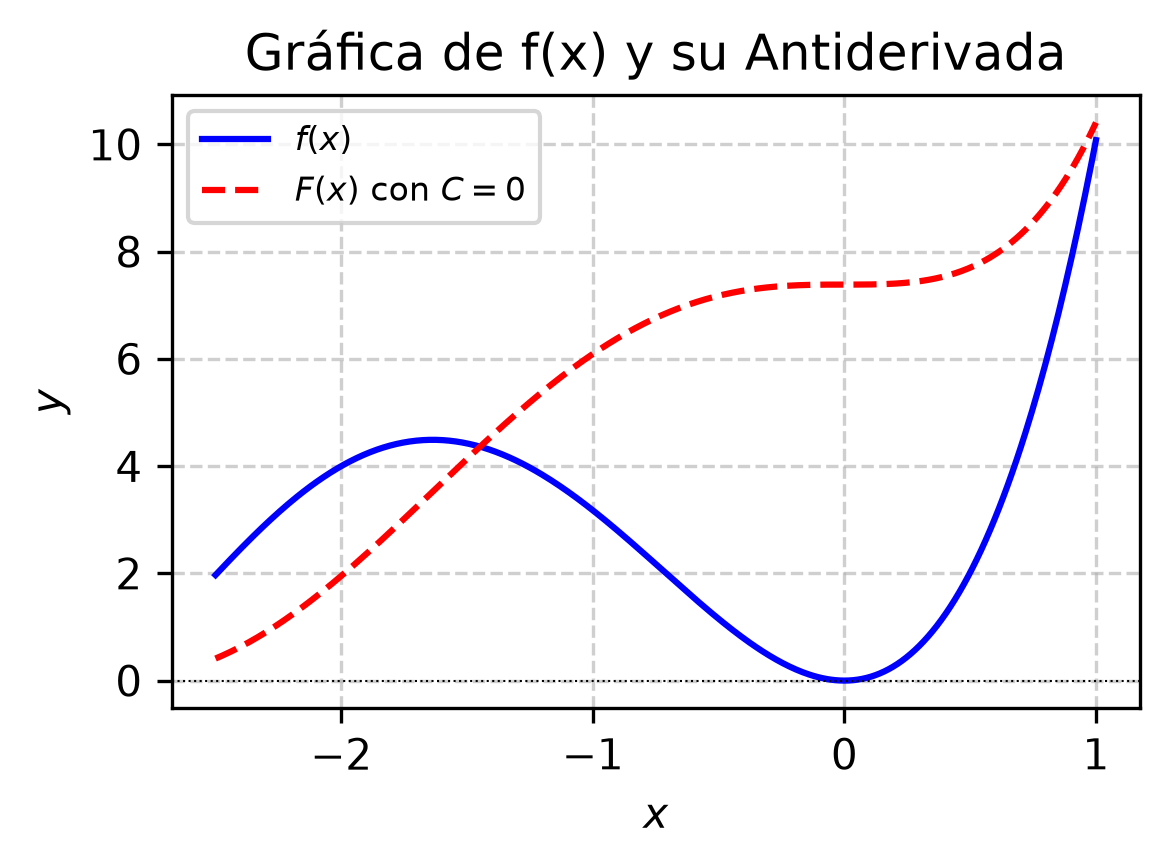
\includegraphics[width=\columnwidth]{semana_05/graficas/SEM05_P39_grafica.png}
	\caption{Representación gráfica de $f(x)$ y su antiderivada $F(x)$ evaluada para la constante de integración $C = 0$ (Problema 39).}
	\label{fig:problema39}
\end{figure}
